%=====================================================================
%  Literature Survey Presentation
%  Privacy-Preserving Recommendation Systems:
%  A Survey of Cryptographic Approaches   (CS670, IIT Kanpur)
%
%  Beamer + Metropolis theme.
%  Compile with:  pdflatex survey_slides.tex   (run twice)
%=====================================================================
\documentclass[10pt,aspectratio=169]{beamer}
 
\usetheme[progressbar=frametitle,numbering=fraction,block=fill,sectionpage=none]{metropolis}
 
\usepackage[T1]{fontenc}
\usepackage{lmodern}
\usepackage{booktabs}
\usepackage{amsmath,amssymb}
\usepackage{tikz}
\usepackage{xspace}
\usetikzlibrary{arrows.meta,positioning,shapes.geometric,fit,backgrounds}
 
% ---- Metropolis colour tweaks: muted, professional ----
\definecolor{mDarkTeal}{HTML}{23373B}
\definecolor{mAccent}{HTML}{0F6E6E}     % teal accent
\setbeamercolor{progress bar}{fg=mAccent}
\setbeamercolor{title separator}{fg=mAccent}
\setbeamercolor{alerted text}{fg=mAccent}
 
% ---- shorthand for system names (small-caps look) ----
\newcommand{\sys}[1]{\textsc{#1}\xspace}
 
% ---- compact table font helper ----
\newcommand{\tbf}[1]{\textbf{#1}}
 
\title{Privacy-Preserving Recommendation Systems}
\subtitle{A Survey of Cryptographic Approaches}
\author{Mainak Sarkar \and Shrasti Dwivedi \and Aditya Anand \and Shravan Agrawal }
\institute{CS670: Cryptographic Techniques for Privacy Preservation\\Indian Institute of Technology Kanpur}
\date{Literature Survey}
 
\begin{document}
 
\maketitle
 
% ---------------------------------------------------------------
\begin{frame}{Outline}
  \setbeamertemplate{section in toc}[sections numbered]
  \tableofcontents[hideallsubsections]
\end{frame}
 
%================================================================
%  PART I
%================================================================
\section{Part I \textbar{} The Problem and the Map}
 
\begin{frame}[standout]
  Part I\\[0.4em]
  {\normalsize The problem, the pipeline, and a taxonomy}
\end{frame}
 
% ---- Motivation ----
\begin{frame}{Why this is a problem}
  Recommender systems are built from the \alert{most revealing data users produce}: what they watched, read, bought and clicked.
 
  \begin{block}{The data is not just sensitive --- it is \emph{identifying}}
    Narayanan \& Shmatikov (2008) de-anonymised the Netflix Prize dataset using IMDb as
    background knowledge, recovering records of known users and their
    ``apparent political preferences and other potentially sensitive information''.
  \end{block}
 
  A large body of work asks: can a recommender be built so that its
  \alert{operator never sees the underlying data}?
 
  Answers come from several communities --- \textbf{secure MPC, PIR, oblivious memory,
  federated learning, differential privacy} --- with different vocabularies,
  threat models, and \emph{parts of the system} they protect.
\end{frame}
 
% ---- The pipeline ----
\begin{frame}{The recommendation pipeline}
  The survey's organising device: a deployed recommender splits into \alert{four stages}.
 
  \vspace{0.6em}
  \begin{center}
  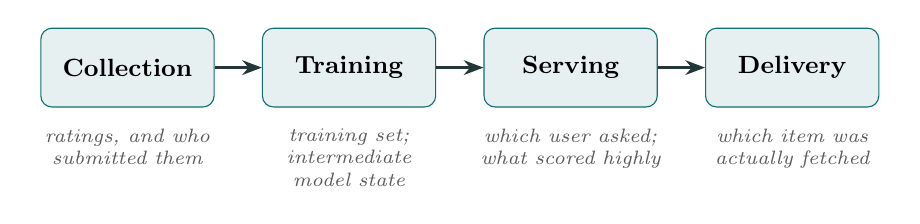
\begin{tikzpicture}[
     node distance=6mm,
     stage/.style={draw, rounded corners, minimum height=1.0cm, minimum width=2.2cm,
                   align=center, font=\small\bfseries, fill=mAccent!10, draw=mAccent},
     lbl/.style={font=\scriptsize\itshape, text width=2.3cm, align=center, text=black!65},
     arr/.style={-{Stealth[length=2.5mm]}, thick, draw=mDarkTeal}]
     \node[stage] (c) {Collection};
     \node[stage, right=of c] (t) {Training};
     \node[stage, right=of t] (s) {Serving};
     \node[stage, right=of s] (d) {Delivery};
     \draw[arr] (c)--(t); \draw[arr] (t)--(s); \draw[arr] (s)--(d);
     \node[lbl, below=1.5mm of c] {ratings, and who submitted them};
     \node[lbl, below=1.5mm of t] {training set; intermediate model state};
     \node[lbl, below=1.5mm of s] {which user asked; what scored highly};
     \node[lbl, below=1.5mm of d] {which item was actually fetched};
  \end{tikzpicture}
  \end{center}
 
  \vspace{0.3em}
  Different lines of work protect different subsets of these stages.
 
  \begin{alertblock}{Consequence}
    A pipeline is only as private as its \emph{weakest stage}. Training under
    secure computation achieves little if the item is then fetched in the clear ---
    the fetch reveals the recommendation.
  \end{alertblock}
\end{frame}
 
% ---- Utility constraint ----
\begin{frame}{Utility constrains the cryptography}
  Recommendation quality is measured by ranking metrics over a held-out set ---
  \alert{nDCG@$k$} and \alert{recall@$k$}.
 
  \begin{itemize}
    \item A private recommender that recommends \emph{badly} has solved nothing.
    \item The constraint propagates into protocol design: \textbf{fixed-point
          arithmetic}, approximation of non-linear functions, and reduced precision
          must not perturb the ranking.
  \end{itemize}
 
  \begin{block}{The core tension}
    Cryptographic primitives compute over rings and finite fields;
    recommendation computes over the \emph{reals}. Bridging that gap is where
    much of the practical cost is incurred.
  \end{block}
 
  Reporting quality \emph{alongside} cost is therefore the norm in this literature.
\end{frame}
 
% ---- Taxonomy: 4 axes ----
\begin{frame}{A taxonomy along four axes}
  Systems are routinely compared as if alternatives --- but they often protect
  \emph{different stages} under \emph{different assumptions}. Four axes make comparison honest:
 
  \vspace{0.4em}
  \begin{columns}[T]
    \column{0.5\textwidth}
      \begin{block}{1. Trust model}
        \footnotesize Who must be trusted? Single server / non-colluding servers /
        federated / trusted hardware.
      \end{block}
      \begin{block}{2. Privacy notion}
        \footnotesize What does ``private'' mean? Cryptographic (simulation)
        / differential privacy / anonymity.
      \end{block}
    \column{0.5\textwidth}
      \begin{block}{3. Pipeline stage protected}
        \footnotesize Collection / Training / Serving / Delivery --- the axis
        the literature is least explicit about.
      \end{block}
      \begin{block}{4. Adversary}
        \footnotesize Semi-honest vs.\ malicious; how many parties may be
        corrupted, and whether fixed in advance.
      \end{block}
  \end{columns}
 
  \vspace{0.5em}
  \begin{center}\small
  \alert{Key idea:} these axes are \textbf{not orderable by strength} --- they are
  different assumptions, not better or worse ones.
  \end{center}
\end{frame}
 
% ---- Taxonomy table (condensed) ----
\begin{frame}{Placing the systems (condensed)}
  \centering\scriptsize
  \renewcommand{\arraystretch}{1.15}
  \begin{tabular}{@{}llccl@{}}
    \toprule
    \tbf{Group / example} & \tbf{Trust model} & \tbf{Notion} & \tbf{Stage} & \tbf{Adversary}\\
    \midrule
    \multicolumn{5}{@{}l}{\emph{Recommendation systems}}\\
    \sys{Pirsona} & $s{+}1$ pairwise n.c. & crypto & C,T,D & semi-honest\\
    \sys{Nudge}   & 3, $\le 1$ corrupt   & crypto & C,T,S & semi-honest\\
    \sys{FedMF}   & federated + HE       & crypto & C,T   & semi-honest\\
    McSherry--Mironov & single server    & DP     & T     & ---\\
    \midrule
    \multicolumn{5}{@{}l}{\emph{Private retrieval / nearest-neighbour}}\\
    \sys{Tiptoe}  & single server        & crypto & S     & semi-honest\\
    \sys{Pacmann} & single server        & crypto & S     & semi-honest\\
    \sys{Compass} & single server        & crypto & S     & compromised svr.\\
    \sys{Wally}   & server-side          & DP     & S     & semi-honest\\
    \midrule
    \multicolumn{5}{@{}l}{\emph{Private information retrieval}}\\
    \sys{SimplePIR}/\sys{Spiral} & single server & crypto & D & semi-honest\\
    Chor et al.\ (multi-server)  & multi-server n.c. & crypto & D & semi-honest\\
    \midrule
    \multicolumn{5}{@{}l}{\emph{Oblivious memory (primitives)}}\\
    \sys{Floram}/\sys{Duoram}/\sys{Prac} & 2--3 party & crypto & --- & semi-honest\\
    \bottomrule
  \end{tabular}
 
  \vspace{0.4em}
  \raggedright\tiny Stages: \textbf{C}ollection, \textbf{T}raining, \textbf{S}erving, \textbf{D}elivery.
  Full 32-system table appears as Table~1 in the report.
\end{frame}
 
% ---- Reading the table ----
\begin{frame}{Three observations from the table}
  \begin{enumerate}
    \item \alert{The stage column is uneven.}\\
      Training and serving are well populated; \emph{delivery} is addressed almost
      entirely by the PIR line in isolation. Only \sys{Pirsona} spans
      collection, training and delivery together.
    \item[]
    \item \alert{Cost is bought with assumptions, consistently.}\\
      The cheapest protocols in each group assume non-collusion. Removing the
      assumption (single-server) normally costs something.
    \item[]
    \item \alert{Semi-honest is the norm at scale.}\\
      Every recommendation system in the table is semi-honest; malicious-security
      exceptions are narrow and not full pipelines.
  \end{enumerate}
\end{frame}
 
%================================================================
%  PART II
%================================================================
\section{Part II \textbar{} Building Blocks and Private Training}
 
\begin{frame}[standout]
  Part II\\[0.4em]
  {\normalsize Cryptographic primitives, and private training}
\end{frame}
 
% ---- Building blocks overview ----
\begin{frame}{Cryptographic building blocks}
  Systems are assembled from a small set of primitives. What matters is each
  one's \alert{cost profile} --- communication, computation, or rounds.
 
  \vspace{0.3em}
  \begin{columns}[T]
    \column{0.5\textwidth}
    \begin{block}{Secret sharing}
      \footnotesize Split a value across parties. Additive (2-party) or replicated
      2-of-3. Addition is free; multiplication needs correlated randomness / rounds.
    \end{block}
    \begin{block}{Garbled circuits}
      \footnotesize Two parties evaluate a Boolean circuit, constant rounds.
      Cost is bandwidth $\propto$ circuit size $\Rightarrow$ binds on data-oblivious algorithms.
    \end{block}
    \begin{block}{Homomorphic encryption}
      \footnotesize Compute on ciphertexts. Enables \emph{single-server} constructions,
      removing non-collusion --- at a computational cost.
    \end{block}
    \column{0.5\textwidth}
    \begin{block}{FSS / distributed point functions}
      \footnotesize Share a \emph{function}. Keys are logarithmic in domain size
      (\emph{compression}) --- makes private read/write layers practical.
    \end{block}
    \begin{block}{Private information retrieval (PIR)}
      \footnotesize Fetch record $j$ without the server learning $j$.
      Multi-server (non-colluding) or single-server (computational).
    \end{block}
    \begin{block}{Oblivious RAM / DORAM}
      \footnotesize Hide \emph{access patterns}. Distributed ORAM for the
      two-party / MPC setting (Floram, Duoram).
    \end{block}
  \end{columns}
\end{frame}
 
% ---- Fixed point ----
\begin{frame}{Fixed-point arithmetic dominates the cost}
  Primitives compute over rings; recommendation computes over the reals.
  A real $v$ is stored as $\lfloor v\cdot 2^t\rfloor$.
 
  \begin{itemize}
    \item Addition is free; a product is $2t$-scaled and must be \alert{truncated} back.
    \item Repeated multiplication needs \alert{normalisation} to stop values growing.
    \item Both are \textbf{non-linear} and expensive under secret sharing.
  \end{itemize}
 
  \begin{block}{Recurring theme}
    Linear algebra is cheap; the non-linear steps are not.
    \sys{SecureML} contributes ``MPC-friendly alternatives to non-linear functions
    such as sigmoid and softmax''; frameworks (ABY, MP-SPDZ) exist precisely because
    different operations are cheapest under different sharings.
  \end{block}
\end{frame}
 
% ---- Private training: garbled circuit era ----
\begin{frame}{Private training (1): the garbled-circuit era}
  Every system here computes the same object: a low-rank factorisation
  $\mathbf{U}\approx\mathbf{A}\cdot\mathbf{B}$ of a rating matrix nobody may see.
 
  \begin{block}{Nikolaenko et al.\ (2013)}
    First practical system --- gradient descent \emph{inside a garbled circuit}
    across two non-colluding servers.
  \end{block}
 
  \alert{Cost profile:} the computation must be data-oblivious, so the circuit is
  sized by the \emph{whole rating matrix} --- \sys{Nudge} reports this family needing
  over four orders of magnitude more communication than secret-sharing approaches.
 
  \begin{center}\small
  \emph{Lesson:} a circuit-based approach pays for every operation in circuit size.
  Secret sharing inverts that relationship.
  \end{center}
\end{frame}
 
% ---- Private training: HE + secret sharing ----
\begin{frame}{Private training (2): HE and the secret-sharing line}
  \begin{block}{Homomorphic encryption --- applied \emph{surgically}}
    \footnotesize
    Removes non-collusion by keeping data encrypted at one server, but FHE of a
    training loop is expensive. \sys{FedMF} uses HE only on the \emph{one channel that
    leaks} (gradient uploads) rather than the whole computation.
  \end{block}
 
  \begin{block}{Secret-sharing MPC --- where the field advanced furthest}
    \footnotesize
    \begin{itemize}
      \item \sys{SecureML} (2 servers): established the pattern; the hard part was
            non-linearities, not linear algebra.
      \item \sys{SecureNN} (3 parties): protocols for ReLU, maxpool, etc.; $6\times$--$113\times$
            faster inference than prior work.
    \end{itemize}
  \end{block}
\end{frame}
 
% ---- Nudge state of the art ----
\begin{frame}{Private training (3): \sys{Nudge} --- the current reference point}
  \sys{Nudge}'s central move is to \alert{change the algorithm}, not just optimise it.
 
  \begin{itemize}
    \item Under 2-of-3 replicated sharing, a matrix--vector product is very cheap.
    \item So it replaces gradient descent with \alert{power iteration} --- mostly
          matrix--vector products, few non-linear steps.
    \item User embeddings $\mathbf{A}$ stay secret-shared; item embeddings $\mathbf{B}$
          are revealed in the clear (a design choice with consequences).
  \end{itemize}
 
  \begin{alertblock}{Headline result --- privacy need not cost accuracy}
    On Netflix (½M users, 10K items), 3$\times$192-core servers:
    trains in 50 min, scoring \textbf{nDCG@20 = 0.29} --- on par with non-private
    matrix factorisation (0.31 for neural). Privacy holds ``against an adversary
    that compromises the entire secret state of one server''.
  \end{alertblock}
\end{frame}
 
% ---- Where each family stops ----
\begin{frame}{Where each training family stops}
  \centering\small
  \renewcommand{\arraystretch}{1.4}
  \begin{tabular}{@{}p{3.4cm}p{7.5cm}@{}}
    \toprule
    \tbf{Family} & \tbf{Stops at\ldots}\\
    \midrule
    Garbled circuits    & \textbf{scale} --- circuit size grows with the data.\\
    Homomorphic enc.\   & \textbf{cost} --- buys single-server, applied to specific channels.\\
    Secret-sharing MPC  & \textbf{the trust assumption} --- fast, but needs 2--3 non-colluding semi-honest parties.\\
    Federated learning  & \textbf{the guarantee} --- gradient uploads leak without an added mechanism.\\
    Differential privacy& \textbf{utility \& scope} --- protects the output, not the computation.\\
    \bottomrule
  \end{tabular}
 
  \vspace{0.8em}
  \begin{center}
  \alert{A limit none of them addresses:} every system ends with a \emph{model or scores}.
  None delivers the recommended \emph{item} --- that is Part III.
  \end{center}
\end{frame}
 
%================================================================
%  PART III
%================================================================
\section{Part III \textbar{} Private Serving, Retrieval and Multi-stage Systems}
 
\begin{frame}[standout]
  Part III\\[0.4em]
  {\normalsize Delivering the item, and composing the pipeline}
\end{frame}
 
% ---- The obstruction ----
\begin{frame}{The obstruction: indices are data-dependent}
  Two problems remain after training: \alert{compute a ranking} without revealing the
  user's profile, and \alert{fetch the item} without revealing which it was.
  Both reduce to \textbf{retrieval} (studied as \emph{private nearest-neighbour search}).
 
  \begin{block}{Why retrieval is hard to hide}
    Retrieval in the clear is fast \emph{because of indices} --- a $k$-d tree, an
    inverted file, a navigable graph. An index is useful precisely because the path
    through it \emph{depends on the query} --- which is exactly what obliviousness forbids.
  \end{block}
 
  \begin{center}\small
  \alert{The organising trade-off:} scan the whole corpus every query (cost linear in
  corpus size), \emph{or} keep the index and hide the traversal (oblivious memory + overhead).
  \end{center}
\end{frame}
 
% ---- Linear scan ----
\begin{frame}{Retrieval approaches (1): linear scan}
  \begin{block}{\sys{Sanns} --- the origin point}
    \footnotesize Secure $k$-NN as ``backbone of recommender systems''; optimised linear
    scan + a sublinear clustering variant, from HE + DORAM + garbled circuits.
    Top-$k$ selection itself is a protocol-design problem.
  \end{block}
 
  \begin{block}{\sys{Tiptoe} --- largest-scale linear approach}
    \footnotesize
    Reduces private full-text search to private nearest-neighbour search with
    semantic embeddings; linearly-homomorphic encryption. \alert{Strongest trust model here}:
    ``based on cryptography alone; no hardware enclaves or non-colluding servers''.
    \\[0.2em]
    45-server cluster, 360M web pages: 145 core-sec compute, 56.9\,MiB comms,
    2.7\,s end-to-end. Ranks best result at position 7.7 (vs.\ 2.3 neural, 6.7 tf-idf).
  \end{block}
\end{frame}
 
% ---- Sublinear / relaxing ----
\begin{frame}{Retrieval approaches (2): index-based and relaxed}
  \begin{columns}[T]
    \column{0.52\textwidth}
    \begin{block}{Sublinear / index-based}
      \footnotesize
      \sys{Pacmann}: moves work \emph{to the client} --- private graph-ANN using the
      preprocessing PIR paradigm. 90\% quality of non-private ANN; up to 62\% less
      compute on 100M vectors.\\[0.3em]
      \sys{Compass}: keeps the index server-side, hides traversal with oblivious memory
      (white-box ORAM co-design). ``Latencies within a second''; privacy of
      ``data, queries, and results, even if the server is compromised''.
    \end{block}
    \column{0.48\textwidth}
    \begin{block}{Relaxing the guarantee}
      \footnotesize
      \sys{Panther}: single-server; co-designs PIR + SS + GC + HE. ANNS query on 10M
      points in 18\,s, 284\,MB --- $7.8\times$ faster, $20\times$ more compact than prior.\\[0.3em]
      \sys{Wally}: relaxes the \emph{privacy notion} to \textbf{differential privacy} to break
      the linear-scan barrier. Batches queries from many clients, each adding
      ``fake queries''. Trust model conventional; notion is DP, not crypto.
    \end{block}
  \end{columns}
  \vspace{0.2em}
  \begin{center}\scriptsize
  \sys{Asharov} et al.: similar-patient genomic search --- shows the \alert{answer itself}
  is sensitive; protecting the computation does not protect the answer.
  \end{center}
\end{frame}
 
% ---- Multi-stage systems ----
\begin{frame}{Systems spanning multiple stages}
  \begin{block}{\sys{Pirsona} --- collection, training \emph{and} delivery}
    \footnotesize
    Treats PIR and collaborative filtering --- ``seemingly antithetical primitives'' ---
    together. Delivery uses multi-server PIR; \alert{collection is folded into delivery}:
    consumption histories are extracted from the query traffic itself (the pipeline
    becomes a \emph{cycle}). Price: strong $s{+}1$-server pairwise non-collusion.
  \end{block}
 
  \begin{block}{\sys{Nudge} --- collection, training and serving}
    \footnotesize
    Users secret-share ratings; servers train and compute scores in shared form.
    Explicit \emph{non-goal}: relies on ``other means (Apple's private relay, Tor, or PIR)''
    for the user to fetch items. Protected up to the point the user \emph{acts}.
  \end{block}
 
  \begin{center}\scriptsize
  \alert{The composition problem:} trust models must agree, party roles need not match,
  and the interface between stages carries information.
  \end{center}
\end{frame}
 
% ---- What the field has and has not built ----
\begin{frame}{What the field has and has not built}
  Reading Table~1 \emph{by column}:
 
  \begin{itemize}
    \item The \textbf{training} stage is well served (Part II).
    \item The \textbf{serving} stage is well served.
    \item \alert{Delivery} is addressed almost entirely by the PIR literature ---
          \emph{in isolation from any recommender}.
  \end{itemize}
 
  \begin{block}{The gap in one sentence}
    Private-retrieval systems take a corpus and embeddings \emph{as given};
    private-training systems produce models and stop. \sys{Pirsona} spans both but
    \emph{predates} that line \emph{almost} in its entirety: \sys{Pirsona} 2021,
    against \sys{Tiptoe} 2023 and \sys{Pacmann}/\sys{Compass}/\sys{Panther}/\sys{Wally}
    2024--2025 --- though \sys{Sanns} (2020) is the one exception.
  \end{block}
 
  We do not claim that composing these lines is straightforward, nor that no
  unpublished work has done so --- only that among the systems surveyed here,
  the two halves are solved \emph{separately}.
\end{frame}
 
%================================================================
%  PART IV
%================================================================
\section{Part IV \textbar{} Evaluation, Open Problems and Conclusion}
 
\begin{frame}[standout]
  Part IV\\[0.4em]
  {\normalsize How the field measures itself, and what remains open}
\end{frame}
 
% ---- Evaluation ----
\begin{frame}{How this literature evaluates itself}
  \begin{columns}[T]
    \column{0.5\textwidth}
    \begin{block}{Datasets}
      \footnotesize MovieLens and Netflix Prize for recommendation;
      MS MARCO / large vector corpora for retrieval. \alert{No shared benchmark}
      spans both halves of the pipeline.
    \end{block}
    \begin{block}{Quality metrics}
      \footnotesize nDCG@$k$, recall@$k$. Best practice: report quality
      \emph{against a non-private baseline} (Nudge: 0.29 vs.\ 0.31; Tiptoe: rank
      7.7 vs.\ 2.3 neural).
    \end{block}
    \column{0.5\textwidth}
    \begin{block}{Cost metrics \& network model}
      \footnotesize Three quantities trade off: \textbf{local computation, bandwidth,
      round complexity}. Which dominates depends entirely on the deployment ---
      a figure without its network model, hardware and dataset is not a result.
    \end{block}
  \end{columns}
 
  \begin{alertblock}{Why cross-paper comparison is unsound}
    Systems differ \emph{simultaneously} in dataset, scale, hardware, network model,
    adversary, non-collusion count and pipeline stage. The survey reports each system in
    \textbf{its authors' own terms} and declines to build a league table.
  \end{alertblock}
\end{frame}
 
% ---- Open problems ----
\begin{frame}{Open problems (from the surveyed authors themselves)}
  \begin{enumerate}
    \item \alert{Malicious security at scale.} Nearly every system at realistic scale is
          semi-honest; the exceptions are narrower than a full pipeline.
    \item \alert{Reducing the non-collusion assumption.} The fastest protocols assume
          non-collusion (about organisations, not mathematics). Single-server at
          competitive cost is open.
    \item \alert{The delivery stage.} Addressed by PIR in isolation; composing it with a
          privately trained recommender is unanswered.
  \end{enumerate}
\end{frame}
 
\begin{frame}{Open problems --- the deepest one}
  \begin{block}{Leakage through the recommendation itself}
    Cryptographic privacy guarantees nothing leaks \emph{beyond the agreed output}.
    But it says nothing about \emph{what the output itself reveals}.
    A recommendation is a statement about the user, delivered to a system that
    observes whether they act on it.
  \end{block}
 
  \begin{itemize}
    \item \sys{Nudge} reveals item embeddings and scores \emph{by design} --- not a flaw,
          but information no in-protocol cryptography would remove.
    \item Differential privacy addresses exactly this class of leak, at a utility cost.
    \item \alert{This is not a protocol failure} --- no improvement in protocol design
          addresses it.
  \end{itemize}
\end{frame}
 
% ---- Direction / conclusion ----
\begin{frame}{The direction we intend to pursue}
  \begin{block}{Our course project}
    Engages with the \alert{composition of a privately trained recommender with a
    private delivery mechanism} --- the gap most visible in Table~1.
  \end{block}
 
  Concretely, the open questions we take from the survey:
  \begin{itemize}
    \item What does it cost to compose a modern private-retrieval backend with a
          privately trained recommender, given the composition obstacles?
    \item Does \sys{Pirsona}'s collection-from-delivery mechanism transfer to a
          \emph{modern} training substrate?
  \end{itemize}
\end{frame}
 
\begin{frame}{Conclusion}
  \begin{center}\large
  Privacy-preserving recommendation is \alert{not one problem but four}, one per pipeline stage.
  \end{center}
 
  \vspace{0.4em}
  \begin{itemize}
    \item \textbf{Training} and \textbf{serving} are in good shape --- crypto privacy costs
          compute and communication, \emph{not} recommendation quality (Nudge: nDCG on par with MF).
    \item \textbf{Delivery} is served by a mature PIR literature that is, with one
          exception, \emph{not connected to any recommender}.
    \item The exception --- \sys{Pirsona} --- shows collection, training and delivery
          \emph{can} be addressed together, but its training core has since been superseded.
    \item The leak carried by the \textbf{recommendation itself} survives any protocol ---
          the most fundamental open problem.
  \end{itemize}
\end{frame}
 
\begin{frame}[standout]
  Thank you\\[0.3em]
  %{\normalsize Questions?}
\end{frame}
 
\end{document}
